% Created by tikzDevice version 0.12 on 2019-05-13 13:11:57
% !TEX encoding = UTF-8 Unicode
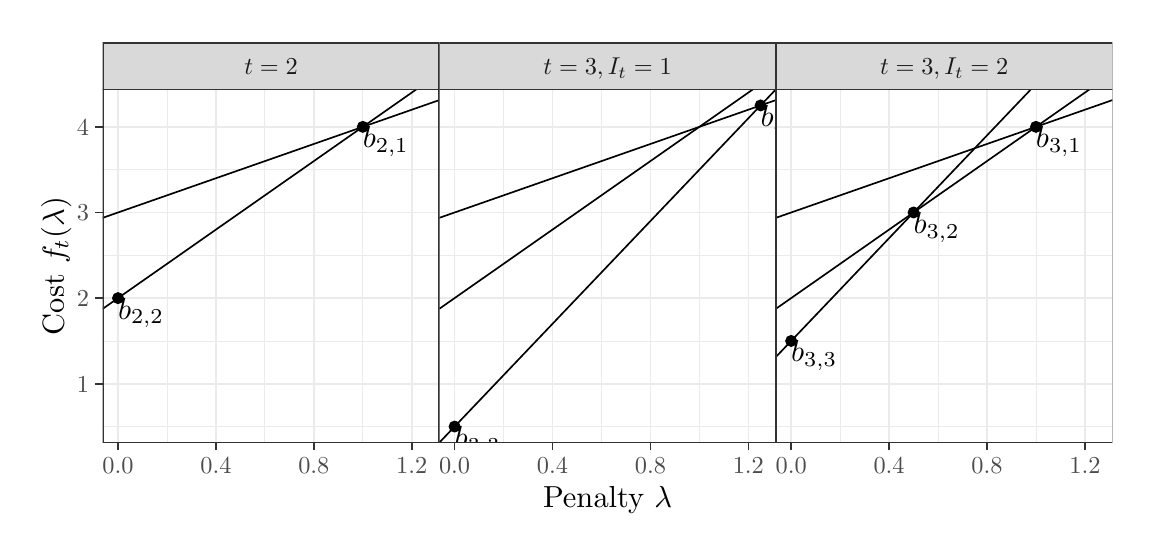
\begin{tikzpicture}[x=1pt,y=1pt]
\definecolor{fillColor}{RGB}{255,255,255}
\path[use as bounding box,fill=fillColor,fill opacity=0.00] (0,0) rectangle (397.48,180.67);
\begin{scope}
\path[clip] (  0.00,  0.00) rectangle (397.48,180.67);
\definecolor{drawColor}{RGB}{255,255,255}
\definecolor{fillColor}{RGB}{255,255,255}

\path[draw=drawColor,line width= 0.6pt,line join=round,line cap=round,fill=fillColor] (  0.00,  0.00) rectangle (397.48,180.67);
\end{scope}
\begin{scope}
\path[clip] ( 27.12, 30.72) rectangle (148.74,158.37);
\definecolor{fillColor}{RGB}{255,255,255}

\path[fill=fillColor] ( 27.12, 30.72) rectangle (148.74,158.37);
\definecolor{drawColor}{gray}{0.92}

\path[draw=drawColor,line width= 0.3pt,line join=round] ( 27.12, 36.53) --
	(148.74, 36.53);

\path[draw=drawColor,line width= 0.3pt,line join=round] ( 27.12, 67.47) --
	(148.74, 67.47);

\path[draw=drawColor,line width= 0.3pt,line join=round] ( 27.12, 98.42) --
	(148.74, 98.42);

\path[draw=drawColor,line width= 0.3pt,line join=round] ( 27.12,129.36) --
	(148.74,129.36);

\path[draw=drawColor,line width= 0.3pt,line join=round] ( 50.34, 30.72) --
	( 50.34,158.37);

\path[draw=drawColor,line width= 0.3pt,line join=round] ( 85.72, 30.72) --
	( 85.72,158.37);

\path[draw=drawColor,line width= 0.3pt,line join=round] (121.10, 30.72) --
	(121.10,158.37);

\path[draw=drawColor,line width= 0.6pt,line join=round] ( 27.12, 52.00) --
	(148.74, 52.00);

\path[draw=drawColor,line width= 0.6pt,line join=round] ( 27.12, 82.94) --
	(148.74, 82.94);

\path[draw=drawColor,line width= 0.6pt,line join=round] ( 27.12,113.89) --
	(148.74,113.89);

\path[draw=drawColor,line width= 0.6pt,line join=round] ( 27.12,144.83) --
	(148.74,144.83);

\path[draw=drawColor,line width= 0.6pt,line join=round] ( 32.65, 30.72) --
	( 32.65,158.37);

\path[draw=drawColor,line width= 0.6pt,line join=round] ( 68.03, 30.72) --
	( 68.03,158.37);

\path[draw=drawColor,line width= 0.6pt,line join=round] (103.41, 30.72) --
	(103.41,158.37);

\path[draw=drawColor,line width= 0.6pt,line join=round] (138.79, 30.72) --
	(138.79,158.37);
\definecolor{drawColor}{RGB}{0,0,0}
\definecolor{fillColor}{RGB}{0,0,0}

\path[draw=drawColor,line width= 0.4pt,line join=round,line cap=round,fill=fillColor] ( 32.65, 82.94) circle (  1.96);

\path[draw=drawColor,line width= 0.4pt,line join=round,line cap=round,fill=fillColor] (121.10,144.83) circle (  1.96);

\node[text=drawColor,anchor=base west,inner sep=0pt, outer sep=0pt, scale=  1.10] at ( 32.65, 75.34) {$b_{2,2}$};

\node[text=drawColor,anchor=base west,inner sep=0pt, outer sep=0pt, scale=  1.10] at (121.10,137.23) {$b_{2,1}$};

\path[draw=drawColor,line width= 0.6pt,line join=round] ( 27.12,111.95) -- (148.74,154.50);

\path[draw=drawColor,line width= 0.6pt,line join=round] ( 27.12, 79.08) -- (148.74,164.17);
\definecolor{drawColor}{gray}{0.20}

\path[draw=drawColor,line width= 0.6pt,line join=round,line cap=round] ( 27.12, 30.72) rectangle (148.74,158.37);
\end{scope}
\begin{scope}
\path[clip] (148.74, 30.72) rectangle (270.36,158.37);
\definecolor{fillColor}{RGB}{255,255,255}

\path[fill=fillColor] (148.74, 30.72) rectangle (270.36,158.37);
\definecolor{drawColor}{gray}{0.92}

\path[draw=drawColor,line width= 0.3pt,line join=round] (148.74, 36.53) --
	(270.36, 36.53);

\path[draw=drawColor,line width= 0.3pt,line join=round] (148.74, 67.47) --
	(270.36, 67.47);

\path[draw=drawColor,line width= 0.3pt,line join=round] (148.74, 98.42) --
	(270.36, 98.42);

\path[draw=drawColor,line width= 0.3pt,line join=round] (148.74,129.36) --
	(270.36,129.36);

\path[draw=drawColor,line width= 0.3pt,line join=round] (171.96, 30.72) --
	(171.96,158.37);

\path[draw=drawColor,line width= 0.3pt,line join=round] (207.34, 30.72) --
	(207.34,158.37);

\path[draw=drawColor,line width= 0.3pt,line join=round] (242.72, 30.72) --
	(242.72,158.37);

\path[draw=drawColor,line width= 0.6pt,line join=round] (148.74, 52.00) --
	(270.36, 52.00);

\path[draw=drawColor,line width= 0.6pt,line join=round] (148.74, 82.94) --
	(270.36, 82.94);

\path[draw=drawColor,line width= 0.6pt,line join=round] (148.74,113.89) --
	(270.36,113.89);

\path[draw=drawColor,line width= 0.6pt,line join=round] (148.74,144.83) --
	(270.36,144.83);

\path[draw=drawColor,line width= 0.6pt,line join=round] (154.27, 30.72) --
	(154.27,158.37);

\path[draw=drawColor,line width= 0.6pt,line join=round] (189.65, 30.72) --
	(189.65,158.37);

\path[draw=drawColor,line width= 0.6pt,line join=round] (225.03, 30.72) --
	(225.03,158.37);

\path[draw=drawColor,line width= 0.6pt,line join=round] (260.41, 30.72) --
	(260.41,158.37);
\definecolor{drawColor}{RGB}{0,0,0}
\definecolor{fillColor}{RGB}{0,0,0}

\path[draw=drawColor,line width= 0.4pt,line join=round,line cap=round,fill=fillColor] (154.27, 36.53) circle (  1.96);

\path[draw=drawColor,line width= 0.4pt,line join=round,line cap=round,fill=fillColor] (264.83,152.57) circle (  1.96);

\node[text=drawColor,anchor=base west,inner sep=0pt, outer sep=0pt, scale=  1.10] at (154.27, 28.92) {$b_{3,3}$};

\node[text=drawColor,anchor=base west,inner sep=0pt, outer sep=0pt, scale=  1.10] at (264.83,144.96) {$b_{3,1}$};

\path[draw=drawColor,line width= 0.6pt,line join=round] (148.74,111.95) -- (270.36,154.50);

\path[draw=drawColor,line width= 0.6pt,line join=round] (148.74, 79.08) -- (270.36,164.17);

\path[draw=drawColor,line width= 0.6pt,line join=round] (148.74, 30.72) -- (270.36,158.37);
\definecolor{drawColor}{gray}{0.20}

\path[draw=drawColor,line width= 0.6pt,line join=round,line cap=round] (148.74, 30.72) rectangle (270.36,158.37);
\end{scope}
\begin{scope}
\path[clip] (270.36, 30.72) rectangle (391.98,158.37);
\definecolor{fillColor}{RGB}{255,255,255}

\path[fill=fillColor] (270.36, 30.72) rectangle (391.98,158.37);
\definecolor{drawColor}{gray}{0.92}

\path[draw=drawColor,line width= 0.3pt,line join=round] (270.36, 36.53) --
	(391.98, 36.53);

\path[draw=drawColor,line width= 0.3pt,line join=round] (270.36, 67.47) --
	(391.98, 67.47);

\path[draw=drawColor,line width= 0.3pt,line join=round] (270.36, 98.42) --
	(391.98, 98.42);

\path[draw=drawColor,line width= 0.3pt,line join=round] (270.36,129.36) --
	(391.98,129.36);

\path[draw=drawColor,line width= 0.3pt,line join=round] (293.58, 30.72) --
	(293.58,158.37);

\path[draw=drawColor,line width= 0.3pt,line join=round] (328.96, 30.72) --
	(328.96,158.37);

\path[draw=drawColor,line width= 0.3pt,line join=round] (364.34, 30.72) --
	(364.34,158.37);

\path[draw=drawColor,line width= 0.6pt,line join=round] (270.36, 52.00) --
	(391.98, 52.00);

\path[draw=drawColor,line width= 0.6pt,line join=round] (270.36, 82.94) --
	(391.98, 82.94);

\path[draw=drawColor,line width= 0.6pt,line join=round] (270.36,113.89) --
	(391.98,113.89);

\path[draw=drawColor,line width= 0.6pt,line join=round] (270.36,144.83) --
	(391.98,144.83);

\path[draw=drawColor,line width= 0.6pt,line join=round] (275.89, 30.72) --
	(275.89,158.37);

\path[draw=drawColor,line width= 0.6pt,line join=round] (311.27, 30.72) --
	(311.27,158.37);

\path[draw=drawColor,line width= 0.6pt,line join=round] (346.65, 30.72) --
	(346.65,158.37);

\path[draw=drawColor,line width= 0.6pt,line join=round] (382.03, 30.72) --
	(382.03,158.37);
\definecolor{drawColor}{RGB}{0,0,0}
\definecolor{fillColor}{RGB}{0,0,0}

\path[draw=drawColor,line width= 0.4pt,line join=round,line cap=round,fill=fillColor] (275.89, 67.47) circle (  1.96);

\path[draw=drawColor,line width= 0.4pt,line join=round,line cap=round,fill=fillColor] (320.12,113.89) circle (  1.96);

\path[draw=drawColor,line width= 0.4pt,line join=round,line cap=round,fill=fillColor] (364.34,144.83) circle (  1.96);

\node[text=drawColor,anchor=base west,inner sep=0pt, outer sep=0pt, scale=  1.10] at (275.89, 59.87) {$b_{3,3}$};

\node[text=drawColor,anchor=base west,inner sep=0pt, outer sep=0pt, scale=  1.10] at (320.12,106.28) {$b_{3,2}$};

\node[text=drawColor,anchor=base west,inner sep=0pt, outer sep=0pt, scale=  1.10] at (364.34,137.23) {$b_{3,1}$};

\path[draw=drawColor,line width= 0.6pt,line join=round] (270.36,111.95) -- (391.98,154.50);

\path[draw=drawColor,line width= 0.6pt,line join=round] (270.36, 79.08) -- (391.98,164.17);

\path[draw=drawColor,line width= 0.6pt,line join=round] (270.36, 61.67) -- (383.75,180.67);
\definecolor{drawColor}{gray}{0.20}

\path[draw=drawColor,line width= 0.6pt,line join=round,line cap=round] (270.36, 30.72) rectangle (391.98,158.37);
\end{scope}
\begin{scope}
\path[clip] ( 27.12,158.37) rectangle (148.74,175.17);
\definecolor{drawColor}{gray}{0.20}
\definecolor{fillColor}{gray}{0.85}

\path[draw=drawColor,line width= 0.6pt,line join=round,line cap=round,fill=fillColor] ( 27.12,158.37) rectangle (148.74,175.17);
\definecolor{drawColor}{gray}{0.10}

\node[text=drawColor,anchor=base,inner sep=0pt, outer sep=0pt, scale=  0.88] at ( 87.93,163.74) {$t=2$};
\end{scope}
\begin{scope}
\path[clip] (148.74,158.37) rectangle (270.36,175.17);
\definecolor{drawColor}{gray}{0.20}
\definecolor{fillColor}{gray}{0.85}

\path[draw=drawColor,line width= 0.6pt,line join=round,line cap=round,fill=fillColor] (148.74,158.37) rectangle (270.36,175.17);
\definecolor{drawColor}{gray}{0.10}

\node[text=drawColor,anchor=base,inner sep=0pt, outer sep=0pt, scale=  0.88] at (209.55,163.74) {$t=3, I_t=1$};
\end{scope}
\begin{scope}
\path[clip] (270.36,158.37) rectangle (391.98,175.17);
\definecolor{drawColor}{gray}{0.20}
\definecolor{fillColor}{gray}{0.85}

\path[draw=drawColor,line width= 0.6pt,line join=round,line cap=round,fill=fillColor] (270.36,158.37) rectangle (391.98,175.17);
\definecolor{drawColor}{gray}{0.10}

\node[text=drawColor,anchor=base,inner sep=0pt, outer sep=0pt, scale=  0.88] at (331.17,163.74) {$t=3, I_t=2$};
\end{scope}
\begin{scope}
\path[clip] (  0.00,  0.00) rectangle (397.48,180.67);
\definecolor{drawColor}{gray}{0.20}

\path[draw=drawColor,line width= 0.6pt,line join=round] ( 32.65, 27.97) --
	( 32.65, 30.72);

\path[draw=drawColor,line width= 0.6pt,line join=round] ( 68.03, 27.97) --
	( 68.03, 30.72);

\path[draw=drawColor,line width= 0.6pt,line join=round] (103.41, 27.97) --
	(103.41, 30.72);

\path[draw=drawColor,line width= 0.6pt,line join=round] (138.79, 27.97) --
	(138.79, 30.72);
\end{scope}
\begin{scope}
\path[clip] (  0.00,  0.00) rectangle (397.48,180.67);
\definecolor{drawColor}{gray}{0.30}

\node[text=drawColor,anchor=base,inner sep=0pt, outer sep=0pt, scale=  0.88] at ( 32.65, 19.71) {0.0};

\node[text=drawColor,anchor=base,inner sep=0pt, outer sep=0pt, scale=  0.88] at ( 68.03, 19.71) {0.4};

\node[text=drawColor,anchor=base,inner sep=0pt, outer sep=0pt, scale=  0.88] at (103.41, 19.71) {0.8};

\node[text=drawColor,anchor=base,inner sep=0pt, outer sep=0pt, scale=  0.88] at (138.79, 19.71) {1.2};
\end{scope}
\begin{scope}
\path[clip] (  0.00,  0.00) rectangle (397.48,180.67);
\definecolor{drawColor}{gray}{0.20}

\path[draw=drawColor,line width= 0.6pt,line join=round] (154.27, 27.97) --
	(154.27, 30.72);

\path[draw=drawColor,line width= 0.6pt,line join=round] (189.65, 27.97) --
	(189.65, 30.72);

\path[draw=drawColor,line width= 0.6pt,line join=round] (225.03, 27.97) --
	(225.03, 30.72);

\path[draw=drawColor,line width= 0.6pt,line join=round] (260.41, 27.97) --
	(260.41, 30.72);
\end{scope}
\begin{scope}
\path[clip] (  0.00,  0.00) rectangle (397.48,180.67);
\definecolor{drawColor}{gray}{0.30}

\node[text=drawColor,anchor=base,inner sep=0pt, outer sep=0pt, scale=  0.88] at (154.27, 19.71) {0.0};

\node[text=drawColor,anchor=base,inner sep=0pt, outer sep=0pt, scale=  0.88] at (189.65, 19.71) {0.4};

\node[text=drawColor,anchor=base,inner sep=0pt, outer sep=0pt, scale=  0.88] at (225.03, 19.71) {0.8};

\node[text=drawColor,anchor=base,inner sep=0pt, outer sep=0pt, scale=  0.88] at (260.41, 19.71) {1.2};
\end{scope}
\begin{scope}
\path[clip] (  0.00,  0.00) rectangle (397.48,180.67);
\definecolor{drawColor}{gray}{0.20}

\path[draw=drawColor,line width= 0.6pt,line join=round] (275.89, 27.97) --
	(275.89, 30.72);

\path[draw=drawColor,line width= 0.6pt,line join=round] (311.27, 27.97) --
	(311.27, 30.72);

\path[draw=drawColor,line width= 0.6pt,line join=round] (346.65, 27.97) --
	(346.65, 30.72);

\path[draw=drawColor,line width= 0.6pt,line join=round] (382.03, 27.97) --
	(382.03, 30.72);
\end{scope}
\begin{scope}
\path[clip] (  0.00,  0.00) rectangle (397.48,180.67);
\definecolor{drawColor}{gray}{0.30}

\node[text=drawColor,anchor=base,inner sep=0pt, outer sep=0pt, scale=  0.88] at (275.89, 19.71) {0.0};

\node[text=drawColor,anchor=base,inner sep=0pt, outer sep=0pt, scale=  0.88] at (311.27, 19.71) {0.4};

\node[text=drawColor,anchor=base,inner sep=0pt, outer sep=0pt, scale=  0.88] at (346.65, 19.71) {0.8};

\node[text=drawColor,anchor=base,inner sep=0pt, outer sep=0pt, scale=  0.88] at (382.03, 19.71) {1.2};
\end{scope}
\begin{scope}
\path[clip] (  0.00,  0.00) rectangle (397.48,180.67);
\definecolor{drawColor}{gray}{0.30}

\node[text=drawColor,anchor=base east,inner sep=0pt, outer sep=0pt, scale=  0.88] at ( 22.17, 48.97) {1};

\node[text=drawColor,anchor=base east,inner sep=0pt, outer sep=0pt, scale=  0.88] at ( 22.17, 79.91) {2};

\node[text=drawColor,anchor=base east,inner sep=0pt, outer sep=0pt, scale=  0.88] at ( 22.17,110.86) {3};

\node[text=drawColor,anchor=base east,inner sep=0pt, outer sep=0pt, scale=  0.88] at ( 22.17,141.80) {4};
\end{scope}
\begin{scope}
\path[clip] (  0.00,  0.00) rectangle (397.48,180.67);
\definecolor{drawColor}{gray}{0.20}

\path[draw=drawColor,line width= 0.6pt,line join=round] ( 24.37, 52.00) --
	( 27.12, 52.00);

\path[draw=drawColor,line width= 0.6pt,line join=round] ( 24.37, 82.94) --
	( 27.12, 82.94);

\path[draw=drawColor,line width= 0.6pt,line join=round] ( 24.37,113.89) --
	( 27.12,113.89);

\path[draw=drawColor,line width= 0.6pt,line join=round] ( 24.37,144.83) --
	( 27.12,144.83);
\end{scope}
\begin{scope}
\path[clip] (  0.00,  0.00) rectangle (397.48,180.67);
\definecolor{drawColor}{RGB}{0,0,0}

\node[text=drawColor,anchor=base,inner sep=0pt, outer sep=0pt, scale=  1.10] at (209.55,  7.44) {Penalty $\lambda$};
\end{scope}
\begin{scope}
\path[clip] (  0.00,  0.00) rectangle (397.48,180.67);
\definecolor{drawColor}{RGB}{0,0,0}

\node[text=drawColor,rotate= 90.00,anchor=base,inner sep=0pt, outer sep=0pt, scale=  1.10] at ( 13.08, 94.55) {Cost $f_t(\lambda)$};
\end{scope}
\end{tikzpicture}
